% Gemini theme
% https://github.com/anishathalye/gemini

\documentclass[final]{beamer}

% ====================
% Packages
% ====================

\usepackage[T1]{fontenc}
\usepackage{lmodern}

% set poster dimensions below (in cm)
% ACIC poster max size is 42" x 42", or 106.68 cm x 106.68 cm
% for a 16/9 aspect ratio, using 
\usepackage[size=custom,width=100,height=56.25,scale=1]{beamerposter}
\usetheme{gemini}
\usecolortheme{mit}
\usepackage{graphicx}
\usepackage{booktabs}

% \usepackage{amsmath}
% \usepackage{amsfonts}
% \usepackage{amsthm}
\usepackage{tikz}
\usepackage{subcaption}
\usepackage{pgfplots}
\pgfplotsset{compat=1.14}
\usepackage{anyfontsize}
\usepackage{hyperref}

\usepackage{hayesmacros}


% \theoremstyle{definition}
% \newtheorem{definition}{Definition}
% \newtheorem{assumption}{Assumption}
% \newtheorem{example}{Example}

% \theoremstyle{plain}
% \newtheorem{proposition}{Proposition}
% \newtheorem{lemma}{Lemma}
% \newtheorem{theorem}{Theorem}
% \newtheorem{corollary}{Corollary}

% \theoremstyle{remark}
% \newtheorem{remark}{Remark}

\hypersetup{colorlinks,allcolors=blue}
\geometry{left=1in,right=1in,top=1in,bottom=1in}

% ====================
% Lengths
% ====================

% If you have N columns, choose \sepwidth and \colwidth such that
% (N+1)*\sepwidth + N*\colwidth = \paperwidth
\newlength{\sepwidth}
\newlength{\colwidth}
\setlength{\sepwidth}{0.025\paperwidth}
\setlength{\colwidth}{0.3\paperwidth}

\newcommand{\separatorcolumn}{\begin{column}{\sepwidth}\end{column}}

% ====================
% Title
% ====================

\title{Estimating network-mediated causal effects via spectral embeddings}

\author{Alex Hayes \inst{1} \and Mark M. Fredrickson \inst{2} \and Keith Levin \inst{1}}

\institute[shortinst]{\inst{1} University of Wisconsin-Madison \samelineand \inst{2} University of Michigan}

% ====================
% Footer (optional)
% ====================

\footercontent{
  \href{https://www.alexpghayes.com}{https://www.alexpghayes.com} \hfill
  % \href{https://www.alexpghayes.com}{https://www.alexpghayes.com} \hfill
  ACIC 2023, Austin, TX \hfill
  \href{mailto:alex.hayes@wisc.edu}{alex.hayes@wisc.edu}}
% (can be left out to remove footer)

% ====================
% Logo (optional)
% ====================

% use this to include logos on the left and/or right side of the header:
\logoright{
\includegraphics[height=7cm]{figures/uw/color-flush-UWlogo-print.pdf}}
% \logoleft{\includegraphics[height=7cm]{logo2.pdf}}

% ====================
% Body
% ====================

\begin{document}

\begin{frame}[t]
\begin{columns}[t]
\separatorcolumn

\begin{column}{\colwidth}

  % \begin{alertblock}{Abstract}

  %   Causal inference for network data is an area of active interest in the social sciences. Unfortunately, the complicated dependence structure of network data presents an obstacle to many causal inference procedures. We consider the task of mediation analysis for network data, and present a model in which mediation occurs in a latent embedding space. Under this model, node-level interventions have causal effects on nodal outcomes, and these effects can be partitioned into a direct effect independent of the network, and an indirect effect induced by homophily. To estimate network-mediated effects, we embed nodes into a low-dimensional space and fit two regression models: (1) an outcome model describing how nodal outcomes vary with treatment, controls, and position in latent space; and (2) a mediator model describing how latent positions vary with treatment and controls. We prove that the estimated coefficients are asymptotically normal about the true coefficients under a sub-gamma generalization of the random dot product graph, a widely-used latent space model. We show that these coefficients can be used in product-of-coefficients estimators for causal inference. Our method is easy to implement, scales to networks with millions of edges, and can be extended to accommodate a variety of structured data.

  % \end{alertblock}

\begin{block}{Motivating example: smoking in adolescent social networks}

    \begin{figure}[ht!]
      \begin{subfigure}{0.49\textwidth}
          \centering
          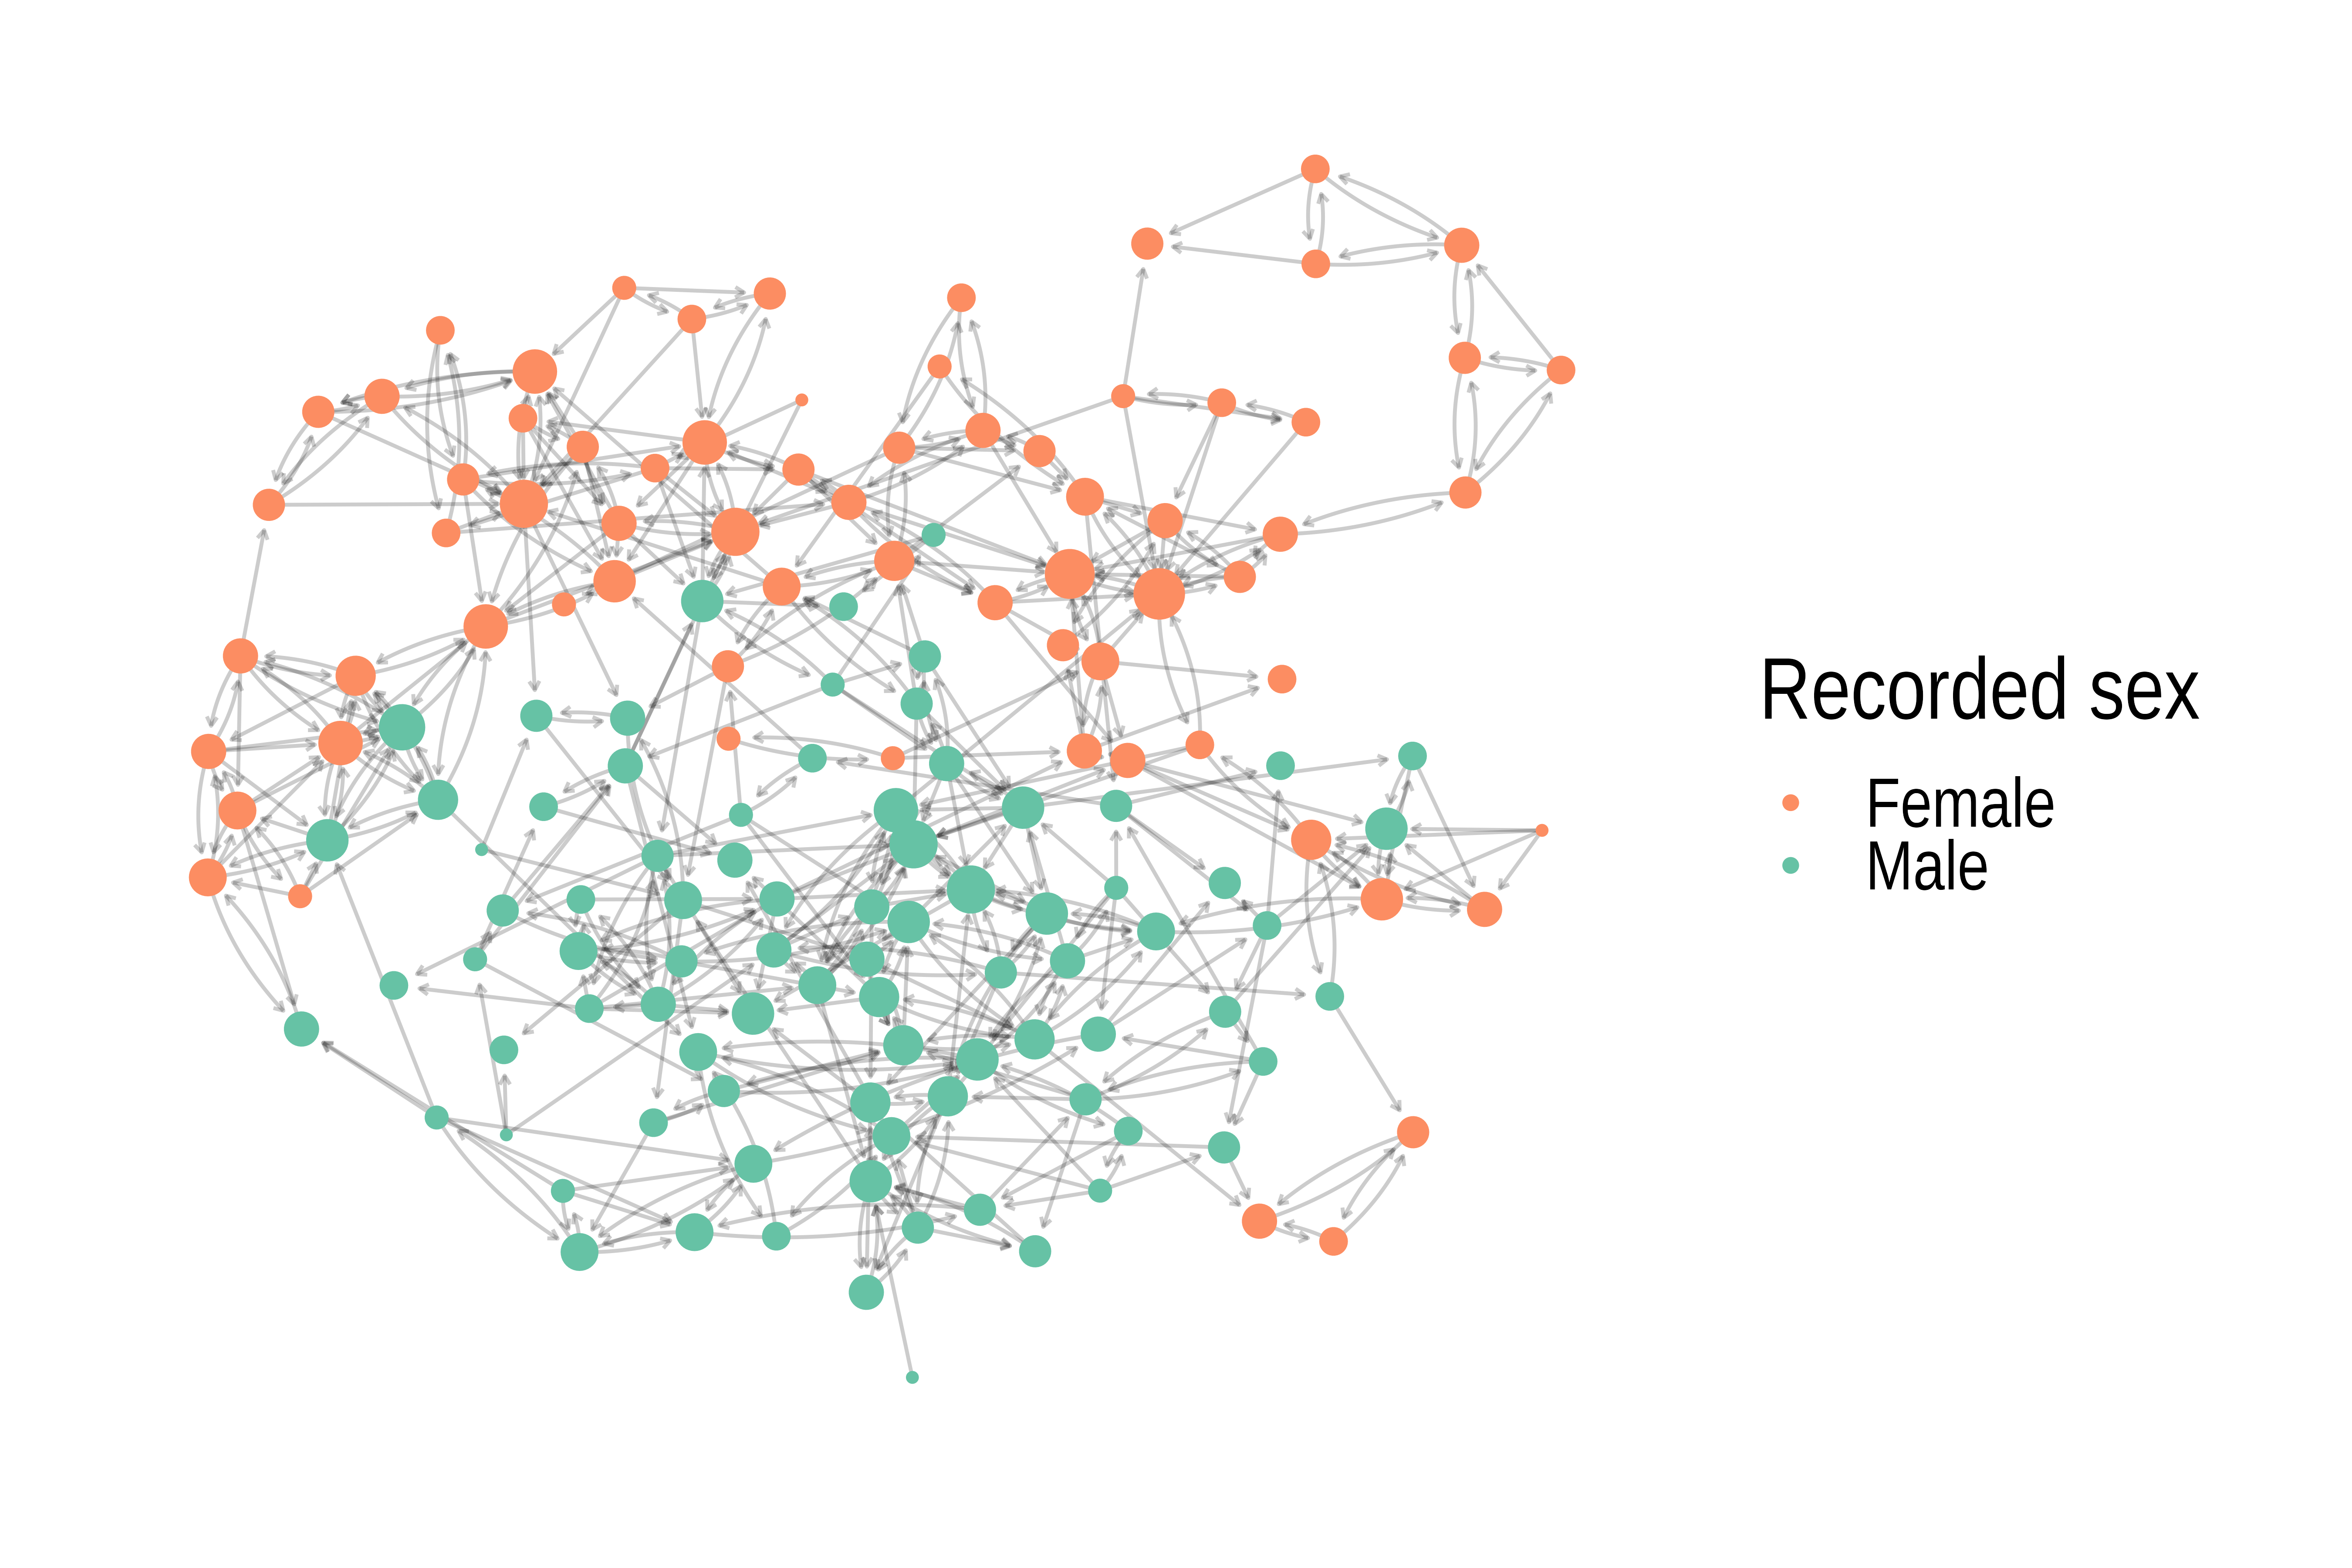
\includegraphics[width=\textwidth]{figures/glasgow/sex.png}
      \end{subfigure}
      \begin{subfigure}{0.49\textwidth}
          \centering
          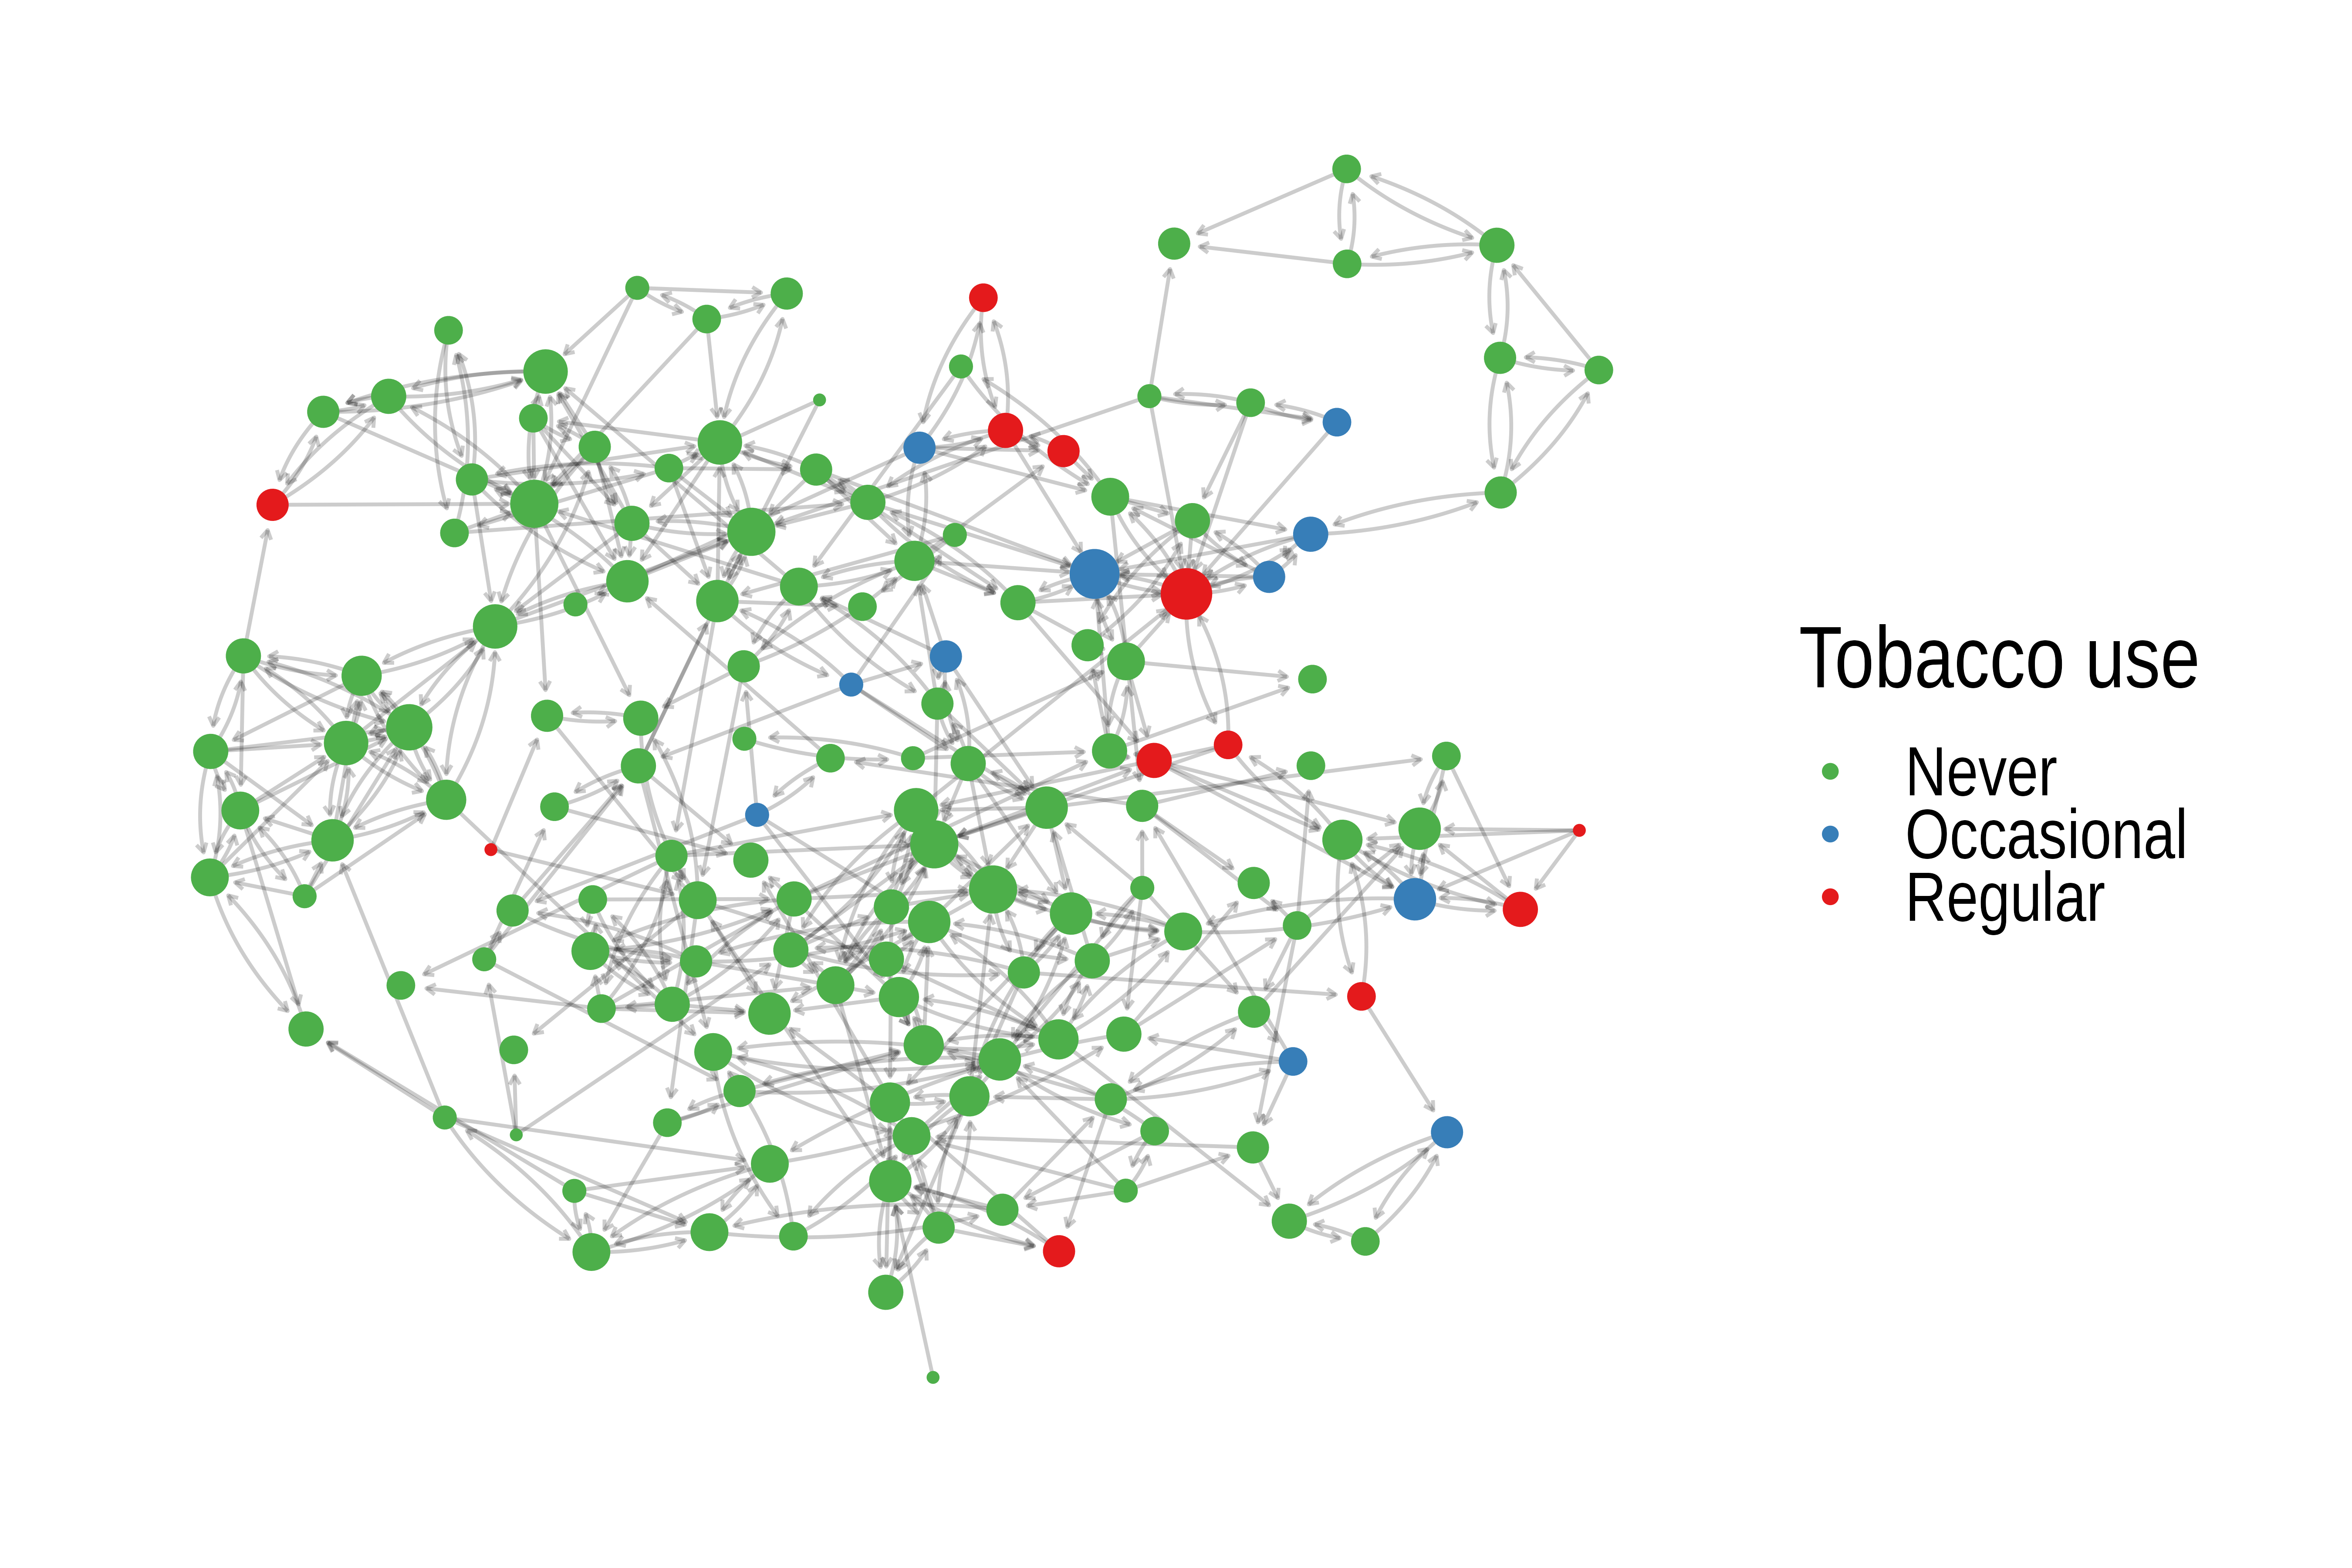
\includegraphics[width=\textwidth]{figures/glasgow/tobacco.png}
      \end{subfigure}
      \caption{Directed friendships in a secondary school in Glasgow, reported in the Teenage Friends and Lifestyle Study (wave 1). Each node represents one student. An arrow from node $i$ to node $j$ indicates student $i$ claimed student $j$ as a friend. Node size is proportional to in-degree. On the left, the network is colored by sex. On the right, the network is colored by self-reported smoking frequency.}
      \label{fig:glasgow}
  \end{figure}
  
\end{block}


\begin{block}{Notation \& inferential targets}

  We assume we have a (symmetric) network with nodes $1, ..., n$.

  \begin{table}[]
    \begin{tabular}{lcc}
    Network   & $A$                    & $\R^{n \times n}$ \\
    Treatment & $T_i$                & $\set{0, 1} $               \\
    Outcome   & $Y_i$                & $\R$                \\
    Confounders & $\C_{i \cdot}$ &  $\R^p$                \\
    Friend group & $\X_{i \cdot}$ & $\R^d$               
    \end{tabular}
  \end{table}

  The \emph{average treatment effect} $\ate$ describes how much the outcome $Y_i$ would change on average if the treatment $T_i$ were changed from $T_i = t$ to $T_i = t^*$:
  \begin{equation*}
      \atef = \E{Y_i(t) - Y_i(t^*)}.
  \end{equation*}
  The \emph{natural direct effect} describes how much the outcome $Y_i$ would change if the exposure $T_i$ were set at level $T_i = t^*$ versus $T_i = t$ but for each individual the mediator $\X_{i \cdot}$ were kept at the level it would have taken for that individual, had $T_i$ been set to $t^*$:
  \begin{equation*}
      \ndef = \E{Y_i(t, \X_{i \cdot}(t^*)) - Y_i(t^*, \X_{i \cdot}(t^*))},
  \end{equation*}
  The \emph{natural indirect effect} describes how much the outcome $Y_i$ would change on average if the exposure were fixed at level $T_i = t^*$ but the mediator $\X_{i \cdot}$ were changed from the level it would take under $T_i = t$ to the level it would take under $T_i = t^*$
  \begin{equation*}
      \nief = \E{Y_i(t, \X_{i \cdot}(t)) - Y_i(t, \X_{i \cdot}(t^*))},
  \end{equation*}

\end{block}

\end{column}

\separatorcolumn

\begin{column}{\colwidth}

  \begin{block}{Structural causal model}

    \begin{figure}[ht]
      \centering
      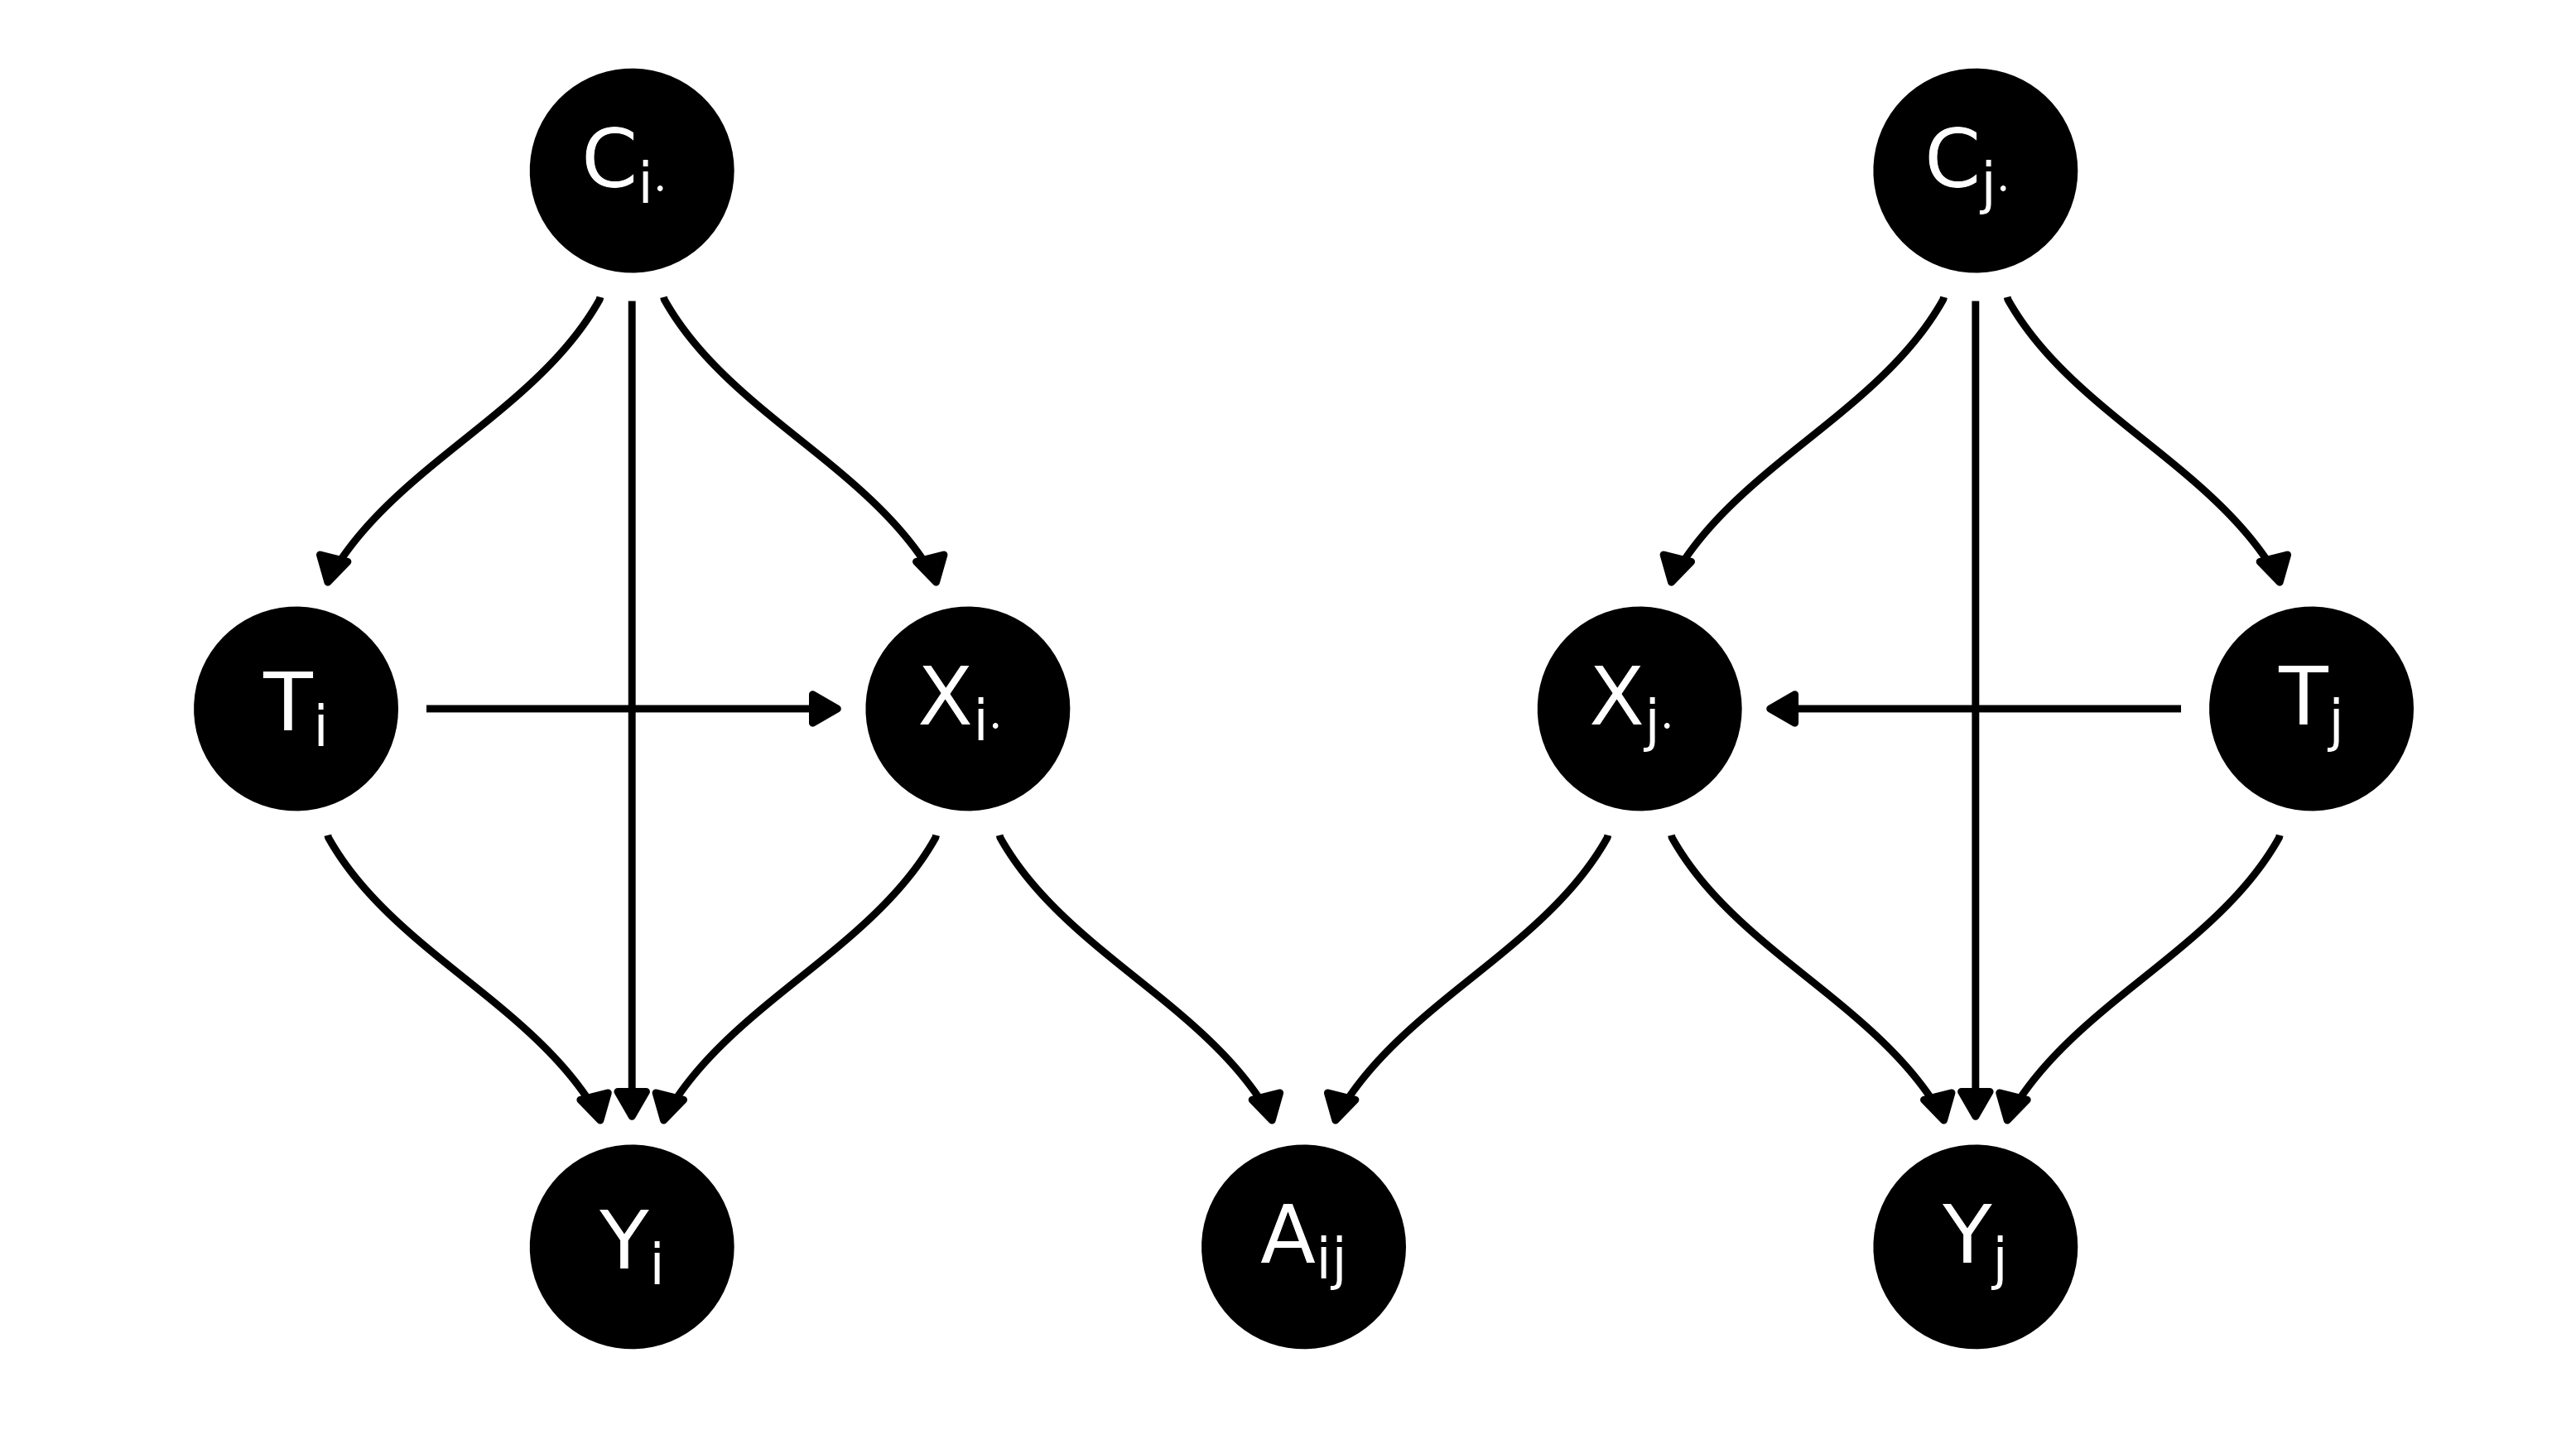
\includegraphics[width=0.6\textwidth]{figures/dags/full_mediating.png}
      \caption{A directed acyclic graph (DAG) representing the causal pathways in a network with homophilous mediation, for node a network with two nodes called $i$ and $j$. We are interested in the causal effect of $T_i$ on $Y_i$ as mediated by the latent position $\X_{i \cdot}$.}
      \label{fig:mediating}
    \end{figure}

  \end{block}

  \begin{block}{Semi-parametric network model}

    Let $A \in \R^{n \times n}$ be a random symmetric matrix, such as the adjacency matrix of an undirected graph. Let $\Apop = \E[\X]{A} = \X \X^T$ be the expectation of $A$ conditional on $\X \in \R^{n \times d}$, which has independent and identically distributed rows $\X_{1 \cdot}, \dots, \X_{n \cdot}$. That is, $\Apop$ has $\rank \paren*{\Apop} = d$ and is positive semi-definite with eigenvalues $\lambda_1 \ge \lambda_2 \ge \cdots \ge \lambda_d > 0 = \lambda_{d+1} = \cdots = \lambda_n$. Conditional on $\X$, the upper-triangular elements of $A - \Apop$ are independent $(\nu_n, b_n)$-sub-gamma random variables.
    
    The outcome regression functional is linear in $T_i, \C_{i \cdot}$, and $\X_{i \cdot}$ and the mediator regression functional is linear in $T_i, \C_{i \cdot}$, and $T_i \cdot \C_{i \cdot}$:
    
    \begin{equation*} 
      \begin{aligned}
            \underbrace{\E[T_i, \C_{i \cdot}, \X_{i \cdot}]{Y_i}}_{\R}
              & = \underbrace{\betazero}_{\R}
            + \underbrace{T_i}_{\{0, 1\}} \underbrace{\betat}_{\R}
            + \underbrace{\C_{i \cdot}}_{\R^{1 \times p}} \underbrace{\betac}_{\R^{p}}
            + \underbrace{\X_{i \cdot}}_{\R^{1 \times d}} \underbrace{\betax}_{\R^d},
              & \text{(outcome model)}                      \\
            \underbrace{\E[T_i, \C_{i \cdot}]{\X_{i \cdot}}}_{\R^{1 \times d}}
              & = \underbrace{\thetazero}_{\R^{1 \times d}}
            + \underbrace{T_i}_{\{0, 1\}} \underbrace{\thetat}_{\R^{1 \times d}}
            + \underbrace{\C_{i \cdot}}_{\R^{1 \times p}} \underbrace{\Thetac}_{\R^{p \times d}}
            + \underbrace{T_i}_{\{0, 1\}} \underbrace{\C_{i \cdot}}_{\R^{1 \times p}} \underbrace{\Thetatc}_{\R^{p \times d}}.
              & \text{(mediator model)}
      \end{aligned}
    \end{equation*}
  \end{block}

  \begin{block}{Semi-parametric causal identification}

    
    Let $\mu_c$ denote the mean of $\C_{i \cdot}$. Then,
    \begin{align*}
        \ndef & = \paren*{t - t^*} \, \betat, ~ \text{ and }                                    \\
        \nief & = \paren*{t - t^*} \, \thetat \, \betax + (t - t^*) \, \mu_c \, \Thetatc \, \betax. 
    \end{align*}

  \end{block}

\end{column}

\separatorcolumn

\begin{column}{\colwidth}
  
  \begin{block}{Estimation challenge: friend groups $\X$ unknown!}
    Given a network with adjacency matrix $A$, the $d$-dimensional \emph{adjacency spectral embedding} (ASE) of $A$ is defined as
    \begin{equation*}
        \Xhat = \Uhat \Shat^{1/2} \in \R^{n \times d},
    \end{equation*}
    where $\Uhat \Shat \Uhat^T$ is the rank-$d$ truncated singular value decomposition of $A$. That is, $\Shat \in \R^{d \times d}$ is diagonal, with entries given by the $d$ leading singular values of $A$, and $\Uhat \in \R^{n \times d}$ has the corresponding $d$ orthonormal singular vectors as its columns.

    Let $\W = \begin{bmatrix} 1 & T & \C \end{bmatrix} \in \R^{n \times (p + 2)}$ and $\Wfull = \begin{bmatrix} W & T \cdot \C \end{bmatrix} \in \R^{n \times (2 p + 2)}$.

    Define $\Dhat = \begin{bmatrix} \W & \Xhat \end{bmatrix} \in \R^{n \times (2 + p + d)}$. We estimate $\betaw$ and $\betax$ via ordinary least squares as follows
    \begin{equation*}
        \begin{bmatrix}
            \betawhat \\
            \betaxhat
        \end{bmatrix}
        = \paren*{\Dhat^T \Dhat}^{-1} \Dhat^T Y.
    \end{equation*}

    Similarly, we estimate $\Theta$ via ordinary least squares as
    \begin{equation*}
        \Thetahat
        = \paren*{\Wfull^T \Wfull}^{-1} \Wfull^T \Xhat.
    \end{equation*}
    
  \end{block}


  \begin{exampleblock}{Theory}

    
    \begin{equation*}
        \begin{aligned}
            \sqrt{ n } \,
            \Sigmahattheta^{-1/2}
            \begin{pmatrix}
                \vecc \paren*{\Thetahat \, Q_n^T} - \Thetavec
            \end{pmatrix}
              & \to
            \Normal{0}{I_{p d}}, \text{ and } \\
            \sqrt{ n } \,
            \Sigmahatbeta^{-1/2}
            \begin{pmatrix}
                \betawhat - \betaw \\
                Q_n \, \betaxhat - \betax
            \end{pmatrix}
              & \to
            \Normal{0}{I_d}.
        \end{aligned}
  \end{equation*}
      
  % \begin{equation*}
  %     \sqrt{n \, \sigmahatnde} \paren*{\ndehat - \nde}
  %     \to
  %     \Normal{0}{1}.
  % \end{equation*}

  % \begin{equation*}
  %     \sqrt{n \, \sigmahatnie} \paren*{\niehat - \nie}
  %     \to
  %     \Normal{0}{1}.
  % \end{equation*}

  \end{exampleblock}

  \begin{block}{Results applied to Glasgow data}

    \begin{figure}[ht!]
      \centering
      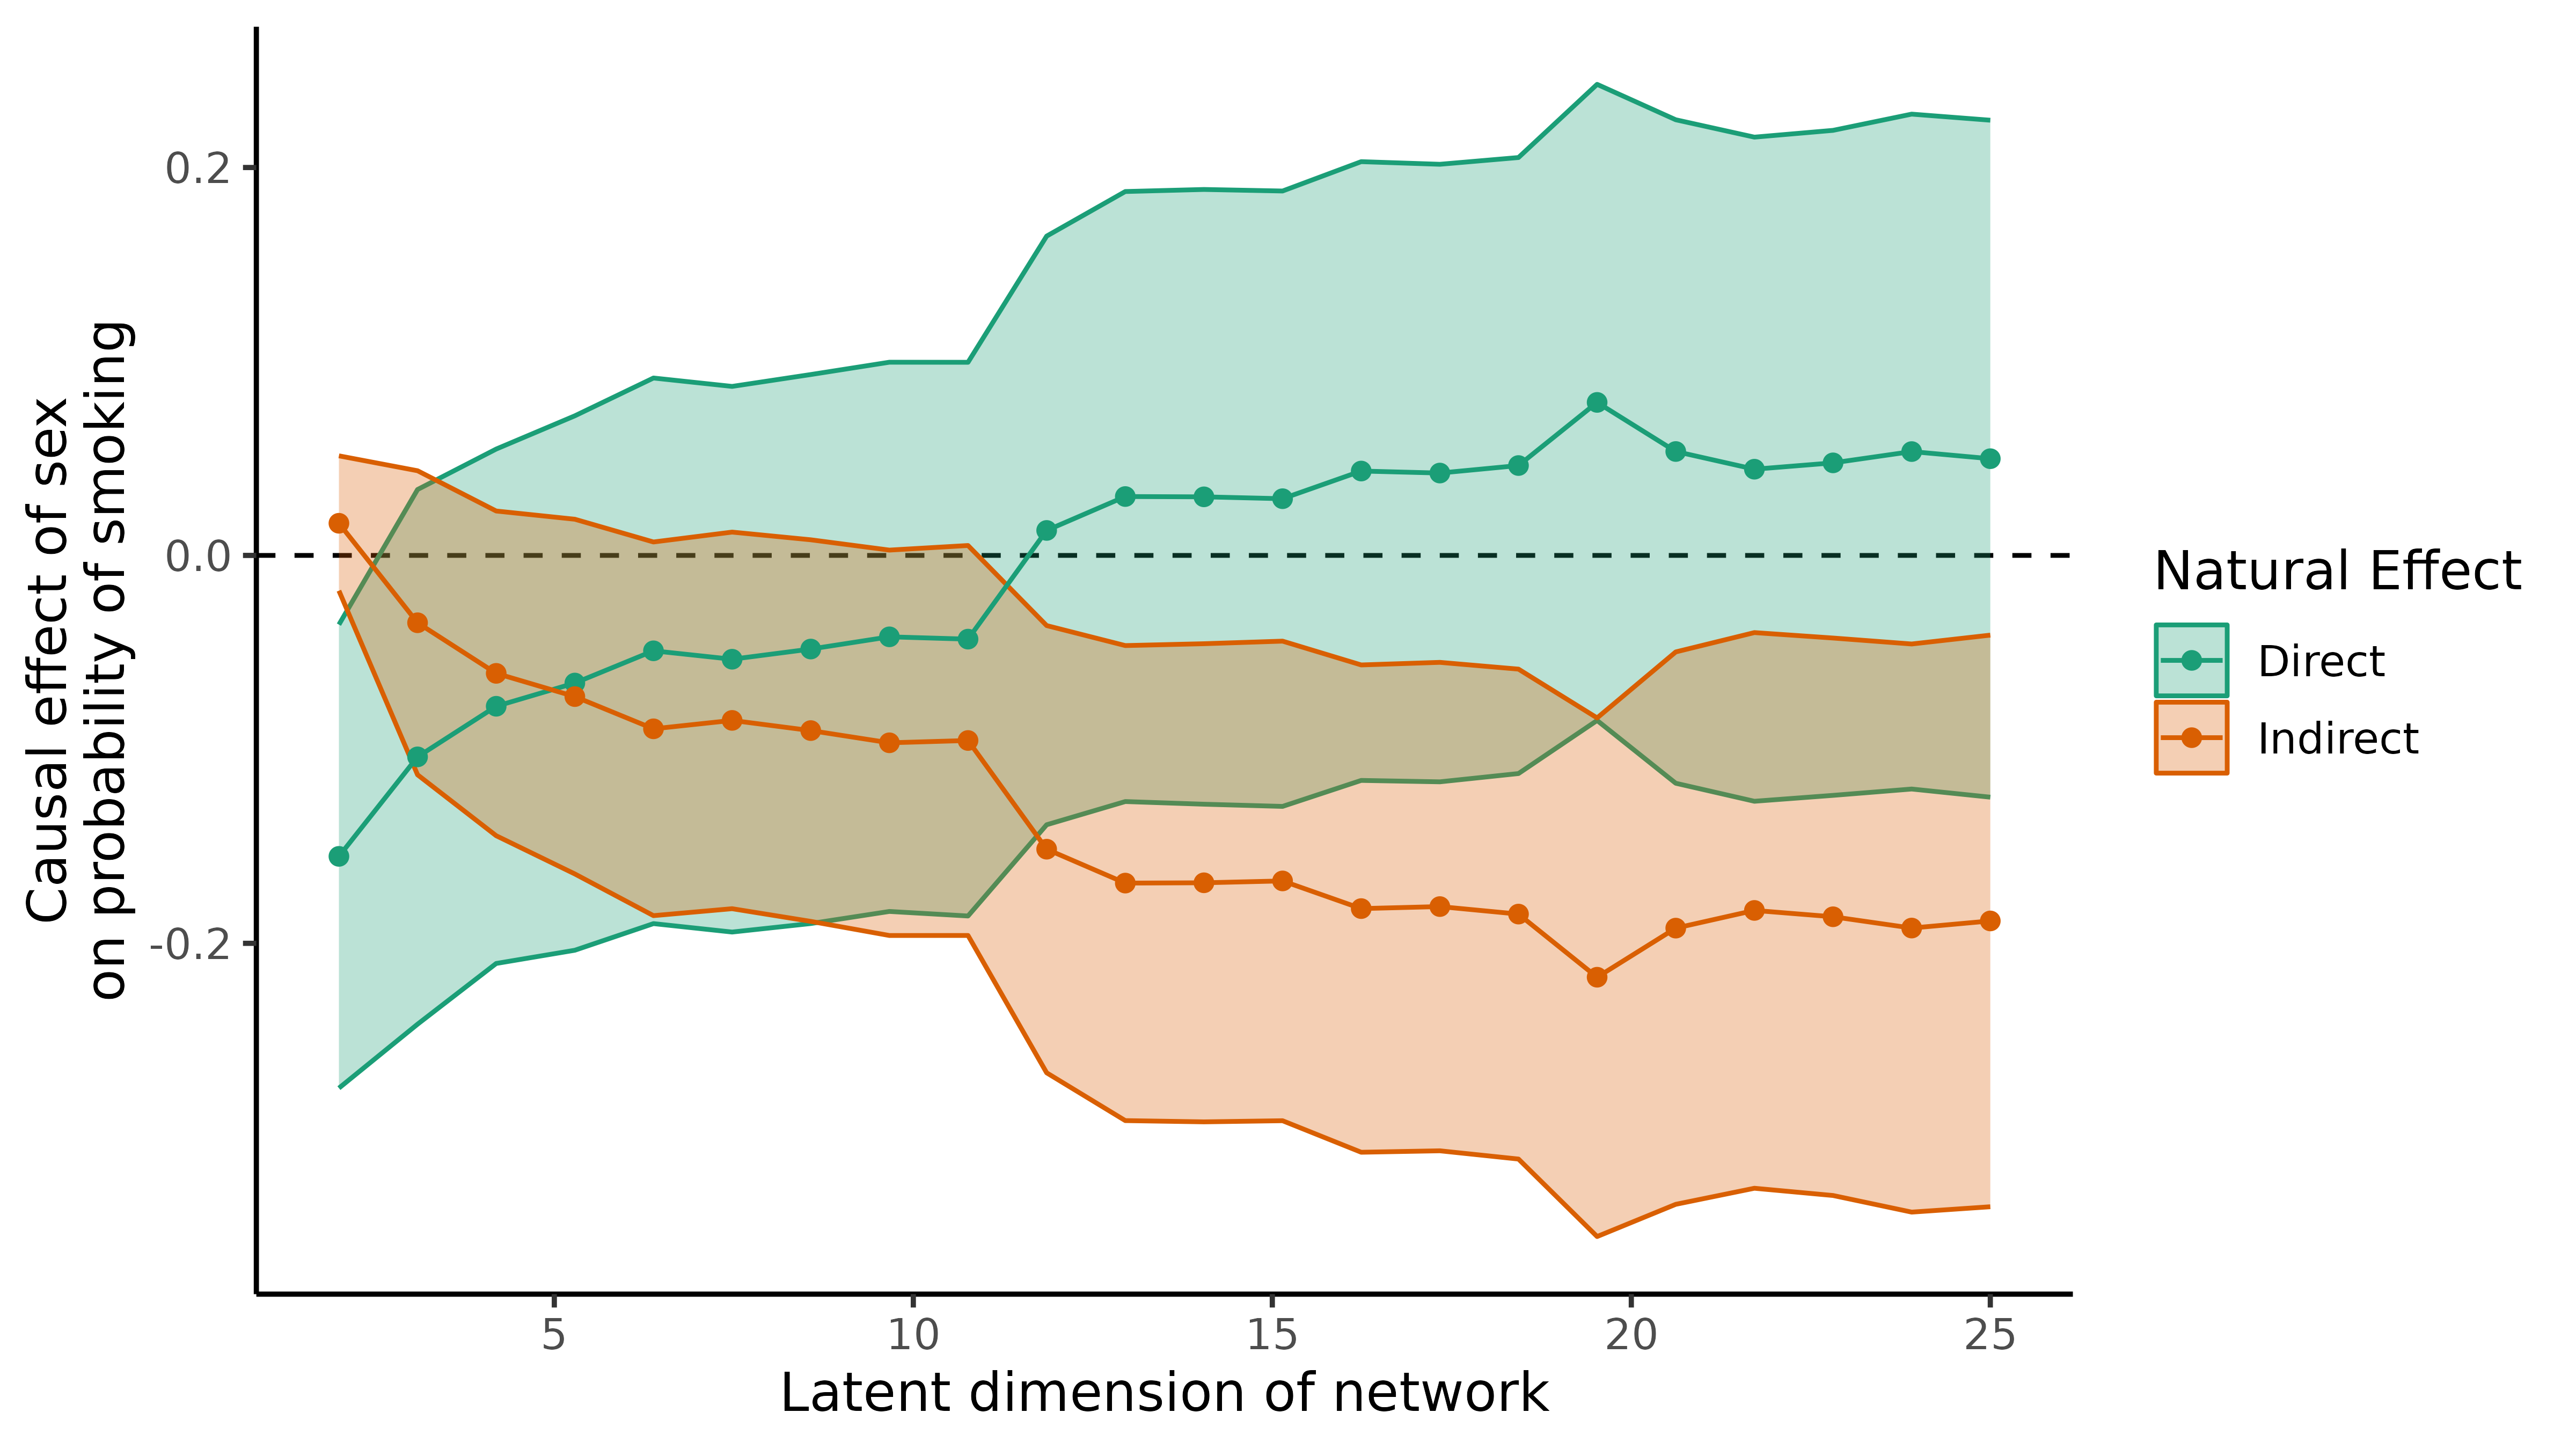
\includegraphics[width=0.5\textwidth]{figures/glasgow/effects.png}
      \caption{Estimated direct and indirect effects of sex on tobacco usage in the Glasgow social network. The estimated effects vary with the dimension $d$ of the latent space, and are adjusted for possibly confounding by age and church attendance. Positive values indicate a greater propensity for adolescent boys to smoke, negative effects a greater propensity for adolescent girls to smoke.}
      \label{fig:glasgow-estimates}
  \end{figure}

  \end{block}

  % \begin{block}{References}

  %   This talk is based on a manuscript recently submitted to JRSS-B, available as a pre-print at https://arxiv.org/abs/2212.12041.

  %   \nocite{*}
  %   \footnotesize{\bibliographystyle{plain}\bibliography{poster}}

  % \end{block}

\end{column}

\separatorcolumn
\end{columns}
\end{frame}

\end{document}
